\documentclass[12pt]{scrartcl}
\usepackage[german, ngerman]{babel}
\usepackage{graphicx}
\usepackage{color}
\usepackage{url}
\usepackage{xcolor}
\usepackage{listings}
\usepackage{hyperref}
\usepackage{nameref}
\usepackage{varioref}
\hypersetup{
    colorlinks=true,
    linkcolor={black!50!black},
    % linkcolor={red!50!black},
    citecolor={black!50!black},
    urlcolor={black!50!black}
}
\usepackage[headsepline,footsepline]{scrlayer-scrpage}
\usepackage{biblatex}
\usepackage{amsmath}
\usepackage{float}
\usepackage{multirow}
\usepackage{multicol}


\newcommand{\code}[1]{\texttt{#1}}


\definecolor{mGreen}{rgb}{0,0.6,0}
\definecolor{mGray}{rgb}{0.5,0.5,0.5}
\definecolor{mPurple}{rgb}{0.58,0,0.82}
\definecolor{backgroundColour}{rgb}{0.95,0.95,0.95} %{cmyk}{0.05,0.05,0.05,0.05}

\lstdefinestyle{CStyle}{
    backgroundcolor=\color{backgroundColour},
    commentstyle=\color{mGreen},
    keywordstyle=\color{blue},
    numberstyle=\tiny\color{mGray},
    stringstyle=\color{mPurple},
    basicstyle=\footnotesize,
    breakatwhitespace=false,
    breaklines=true,
    captionpos=b,
    keepspaces=true,
    numbers=left,
    numbersep=5pt,
    showspaces=false,
    showstringspaces=false,
    showtabs=false,
    tabsize=2,
    language=C++
}

\lstdefinestyle{Terminal}{
    backgroundcolor=\color{backgroundColour},
    commentstyle=\color{black},
    keywordstyle=\color{black},
    numberstyle=\tiny\color{black},
    stringstyle=\color{black},
    basicstyle=\footnotesize,
    breakatwhitespace=false,
    breaklines=true,
    captionpos=b,
    keepspaces=true,
    numbers=none,
    numbersep=5pt,
    showspaces=false,
    showstringspaces=false,
    showtabs=false,
    tabsize=2,
}


\pagestyle{scrheadings}
\clearscrheadfoot
%\cfoot{Tobias Gruber}
\cfoot{\pagemark}
\chead{\headmark}
\automark[subsection]{section}


\begin{document}


\begin{titlepage}
    \vfill
	\centering
    \vspace{1.5cm}

	{\scshape\LARGE Hochschule München \par}
    {\scshape\Large Fakultät für Informatik und Mathematik\par}
	\vspace{1.5cm}




    \vfill
    {\LARGE\bfseries Praktikumsaufgabe 5 \\}
    \vspace{0.5cm}
	{in der Vorlesung\\}
    \vspace{0.5cm}
    {\LARGE\bfseries Computational Geometry\\~\\ \par}
	{\LARGE Größter Inkreis eines Polygons\\~\\ \par}
	\vfill
    \vfill


    \begin{tabular}{ll}
    \normalsize
    Team:  & Christopher Hinz, Tobias Gruber\\
    Studiengruppe: & Master Informatik\\
    Studiensemester: & 1. Semester\\
    Schwerpunkt: & Embedded Computing\\
    \end{tabular}
    \vspace{1.5cm}

    \today

    \vspace{0.5cm}

    Sommersemester 2022

	\vfill

\end{titlepage}

\newpage

%%%%%%%%%%%%%%%%%%%%%%%%%%%%%
% Einführung
%%%%%%%%%%%%%%%%%%%%%%%%%%%%%
\section{Einführung}
Es soll für ein gegebenes konvexes Polygon der größte Inkreis mittels Linear Programming gefunden werden.
Als Plattform zur Lösung des Problems wird die Entwicklungsumgebung Matlab verwendet.

%%%%%%%%%%%%%%%%%%%%%%%%%%%%%
% Zielfunktion
%%%%%%%%%%%%%%%%%%%%%%%%%%%%%
\section{Zielfunktion}
Um ein Problem mittels Linear Programming lösen zu können, muss eine Zielfunktion, sowie die Randbedingungen vorgegeben werden.
Ein Kreis lässt sich mittels drei Parameter beschreiben. Diese sind die x- und y-Koordinaten des Mittelpunktes, sowie der Radius des Kreises.

\begin{equation}
    k = \begin{pmatrix} x_0 \\ y_0 \\ r \end{pmatrix}
\end{equation}

Ziel ist es den Kreis so groß wie möglich zu machen.
Als Zielfunktion für den größten Inkreis eines Polygons wird somit der Radius gewählt, da dieser maximiert werden soll. Da der Mittelpunkt des Kreises beliebig ist, kann die Zielfunktion wie folgt formuliert werden:

\begin{equation}
    c^T = \begin{pmatrix} 0 \\ 0 \\ 1 \end{pmatrix}
\end{equation}

Durch Multiplikation des Kreisvektors mit der Zielfunktion erhält man somit ausschließlich den Radius.

\begin{equation}
    c^T \cdot k = \begin{pmatrix} 0 \\ 0 \\ 1 \end{pmatrix} \cdot \begin{pmatrix} x_0 \\ y_0 \\ r \end{pmatrix} = r
\end{equation}

%%%%%%%%%%%%%%%%%%%%%%%%%%%%%
% Randbedingungen
%%%%%%%%%%%%%%%%%%%%%%%%%%%%%
\section{Randbedingungen}
Ohne Randbedingungen könnte nun der Radius des Kreises unendlich groß gewählt werden.
Die Größe des Kreises wird jedoch durch die Kanten des Polygons begrenzt.
Da das Ziel ist die Kanten des Polygons mit dem Kreis zu tangieren, kann man den Radius des Kreises auch als Abstand des Mittelpunktes des Kreises zu den Kanten des Polygons verstehen.

\subsection{Aufstellen der Hesseschen Normalenform}
Zur Messung des Abstands eines Punktes zu einer Stecke bietet sich die Verwendung der Hesseschen Normalenform an.
Die Hessesche Normalenform beschreibt die Gerade $g$, auf der die Kante des Polygons liegt mit dem normierten Normalenvektor $\vec{n} =  \begin{pmatrix} n_x \\ n_y \end{pmatrix}$ auf die Gerade, sowie dem kürzesten Abstand $d$ der Gerade zum Nullpunkt.

\begin{equation}
    g: n_x \cdot x + n_y \cdot y + d = 0
\end{equation}

Die Hessesche Normalenform lässt sich aus den beiden Eckpunkten $p$ und $q$ des Polygons, die eine Kante bestimmen formulieren.
Hierfür wird ein Gleichungssystem mit durch zwei Bedingungen aufgestellt.
Als erste Bedingung wird festgelegt, dass der Normalenvektor $\vec{n}$ senkrecht auf den Richtungsvektor der Eckpunkte stehen soll. Diese Bedingung lässt sich mit dem Skalarprodukt beider Vektoren ausdrücken.

\begin{equation}
    \vec{n} \cdot \vec{pq} = (q_x - p_x) \cdot n_x + (q_y - p_y) \cdot n_y = 0
\end{equation}

Die zweite Bedingung lautet, dass der Normalenvektor normiert sein soll, also die Länge 1 besitzt.

\begin{equation}
    |\vec{n}| = \sqrt{n_x^2 + n_y^2} = 1
\end{equation}

Mit diesen Bedingungen lässt sich das Gleichungssystem bereits lösen.
Man erhält jedoch zwei Lösungen, da der normierte Normalenvektor auf beiden Seiten der Gerade liegen kann.
Zur Messung des Abstands des Kreismittelpunktes zur Geraden der Polygonkante soll der Normalenvektor verwendet werden, der zum Inneren des Polygons zeigt.
Da es sich um ein konvexes Polygon handelt, kann der zur Innenseite des Polygons gerichtete Normalenvektor über die Koordinaten der Eckpunkte der Kanten bestimmt werden.

\begin{figure}[ht]
    \centering
    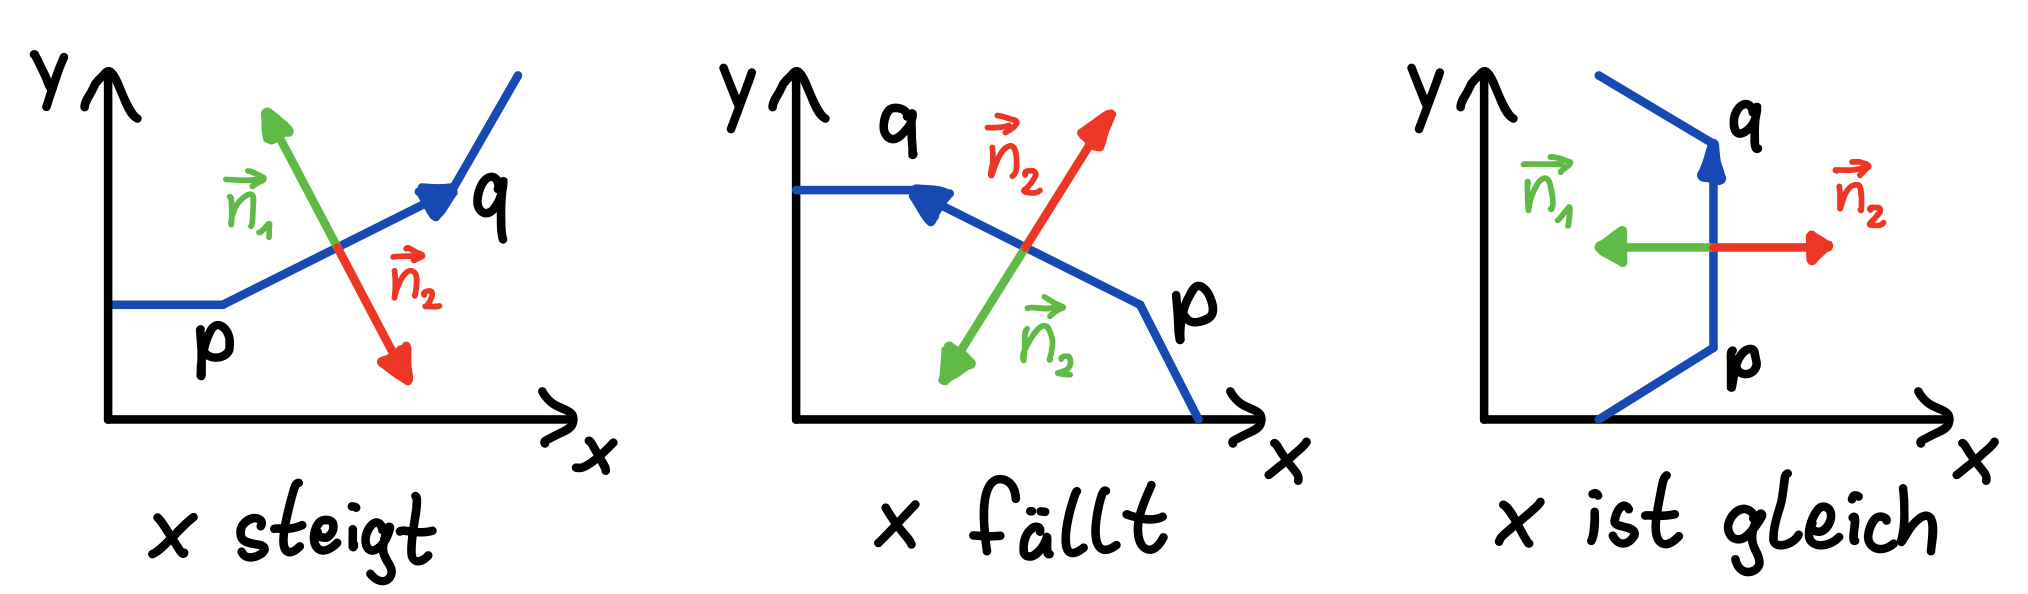
\includegraphics[scale=0.2]{Auswahl Normalenvektor.png}
    \caption{Fallunterscheidung zur Auswahl des korrekten Normalenvektors.}
    \label{fig:auswahlNormvek}
\end{figure}

\autoref{fig:auswahlNormvek} zeigt die Auswahl des Normalenvektors nach drei Entscheidungskriterien.
\begin{itemize}
    \item Steigt die x-Komponente des Richtungsvektors $\vec{pq}$ an, so wird der Normalenvektor mit positiver y-Komponente gewählt.
    \item Fällt die x-Komponente des Richtungsvektors $\vec{pq}$ ab, so wird der Normalenvektor mit negativer y-Komponente gewählt.
    \item Enthält die x-Komponente des Richtungsvektors $\vec{pq}$ den Wert Null, so wird die Entscheidung entsprechend anhand der y-Komponente des Richtungsvektors und der x-Komponente des Normalenvektors getroffen.
\end{itemize}

In einem weiteren Schritt wird der Parameter $d$ der Geradengleichung nach der Hesseschen Normalenform bestimmt.
Dieser kann durch einsetzen des Normalenvektors, sowie eines der beiden Eckpunkte in die Hessesche Normalenform bestimmt werden.

\begin{equation}
    d = -n_x \cdot p_x - n_y \cdot p_y
\end{equation}

Die Berechnungen werden für alle Kanten des Polynoms durchgeführt.
Damit sind alle benötigten Parameter für die Randbedingungen gefunden.
Nun muss noch aus den formulierten Normalengleichungen die Randbedingung für die Lösung mittels Linear Programming formuliert werden.

\subsection{Formulierung der Randbedingungen}
Wie bereits erwähnt, wird die Normalenform verwendet, um den Abstand der Kante vom Mittelpunkt des Kreises zu berechnen. Die Formel zur Berechnung des Abstands $r$ eines Punktes zu einer Geraden in Hessen Normalenform lautet:

\begin{equation}
    r = n_x \cdot x_0 + n_y \cdot y_0 - d
\end{equation}

Für gewöhnlich müsste hier der Betrag des rechten Terms verwendet werden, da sich ein Punkt theoretisch auf beiden Seiten der Gerade befinden kann. Da wir aber nur eine Lösung für Kreise innerhalb der Polygons erhalten wollen und den Normalenvektor entsprechend gewählt haben, wird hier nicht weiter der Betrag der Funktion benötigt.

Die Gleichung enthält nun schon alle Parameter des Kreises als Variable und kann daher als Randbedingung verwendet werden.
Zunächst muss die Gleichung noch zu einer Ungleichung erweitert werden, da der Radius des Kreises kleiner oder gleich sein muss, wie der berechnete Abstand des Mittelpunktes zur Geraden.

\begin{equation}
    r \leq n_x \cdot x_0 + n_y \cdot y_0 - d
\end{equation}

Zur Lösung des Problems mittels Linear Programming wird nun noch die Ungleichung so umgestellt, dass der linke Term die Parameter des Kreises und der rechte Term ausschließlich eine Konstante enthält.

\begin{equation}
    -n_x \cdot x_0 - n_y \cdot y_0 + r \leq - d
\end{equation}

Für jede Kante des Polygons wird nun eine Randbedingung aufgestellt und alle Ergebnisse in der Koeffizientenmatrix $A$ und im Konstanten-Vektor $b$ gespeichert.
Das System kann nun mittels LP-Solver nach folgender Form gelöst werden:

\begin{equation}
    \max\{c^T \cdot x | Ax \leq b, x \geq 0\}
\end{equation}

\section{Ergebnisse}
Die Umsetzung des Algorithmus liefert ein korrektes Ergebnis für den Testdatensatz, sowie eine plausible Lösung für das zu untersuchende Polynom.
Für den Testdatensatz lautet das Ergebnis der Berechnung:

\begin{figure}[ht]
    \centering
    \begin{minipage}[c]{8cm}
        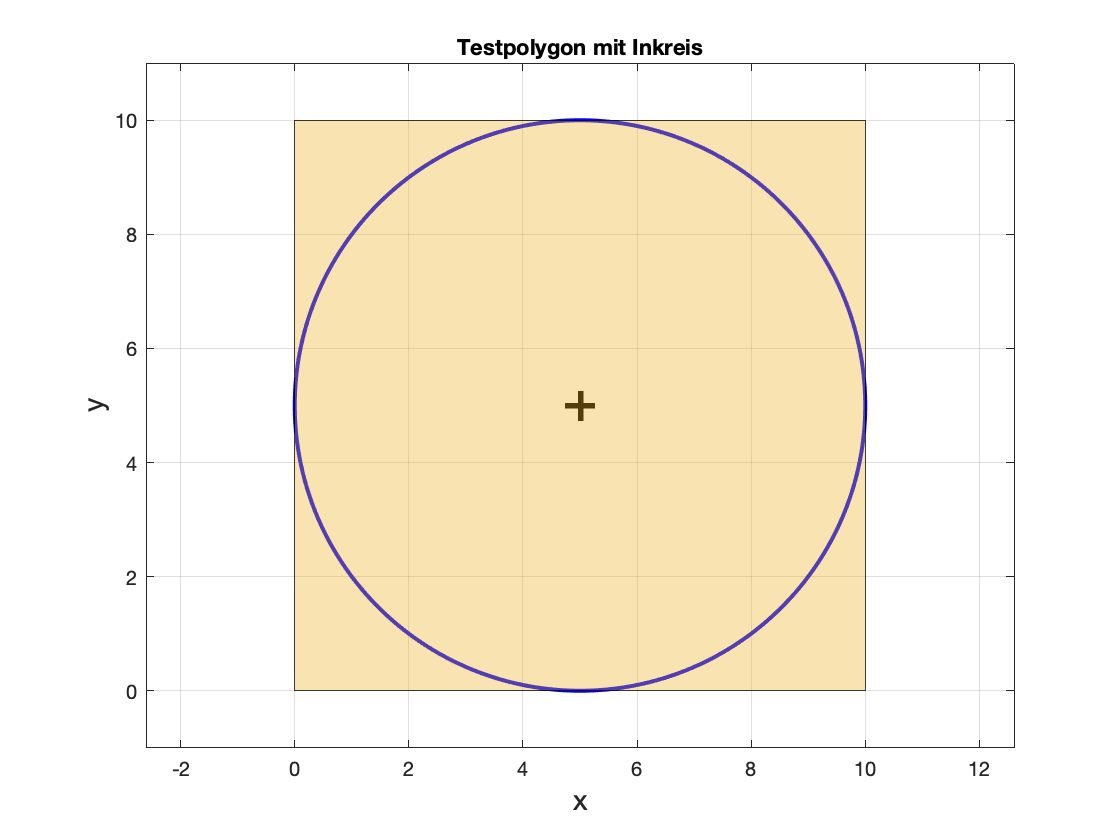
\includegraphics[width=8cm]{Testpolygon.png}
    \end{minipage}%
    \begin{minipage}[c]{6cm}
        \begin{equation}
            k_{test} = \begin{pmatrix} x_0 \\ y_0 \\ r \end{pmatrix} = \begin{pmatrix} 5 \\ 5 \\ 5 \end{pmatrix}
        \end{equation}
    \end{minipage}
    \caption{Plot des Testpolygons mit größtmöglichem Inkreis}
    \label{fig:Testpolygon}
\end{figure}

Das Ergebnis für das zu untersuchende Polynom lautet:

\begin{figure}[ht]
    \centering
    \begin{minipage}[c]{8cm}
        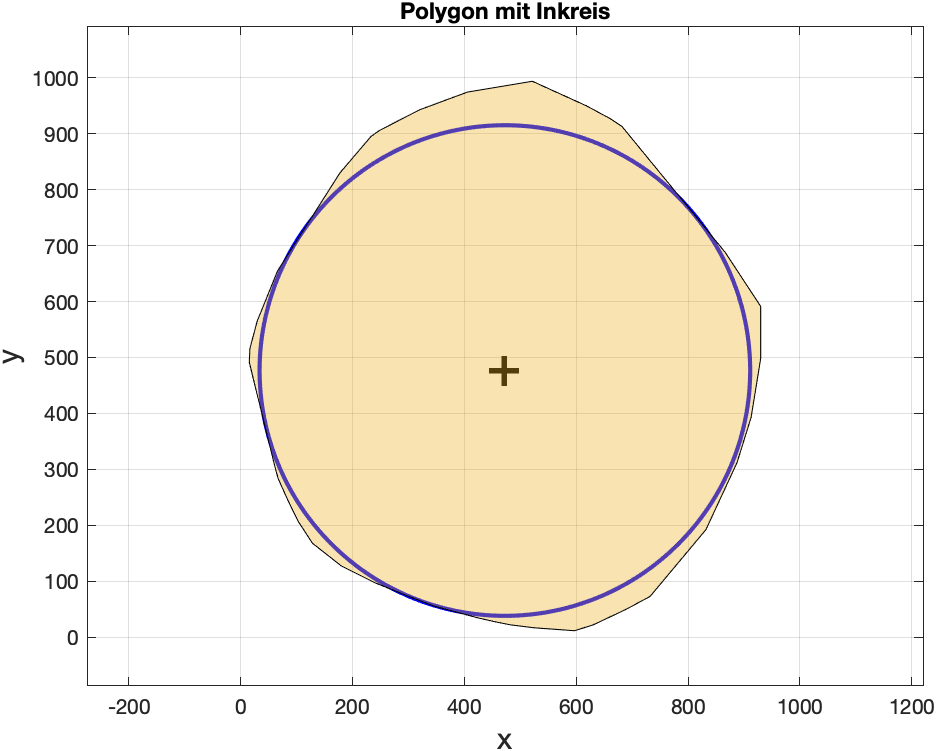
\includegraphics[width=8cm]{Polygon.png}
    \end{minipage}%
    \begin{minipage}[c]{7cm}
        \begin{equation}
            k_{poly} = \begin{pmatrix} x_0 \\ y_0 \\ r \end{pmatrix} = \begin{pmatrix} 472.5705 \\ 476.6642 \\ -438.5922 \end{pmatrix}
        \end{equation}
    \end{minipage}
    \caption{Plot des zu untersuchenden Polygons mit größtmöglichem Inkreis}
    \label{fig:Polygon}
\end{figure}

%\begin{figure}[ht]
%    \centering
%    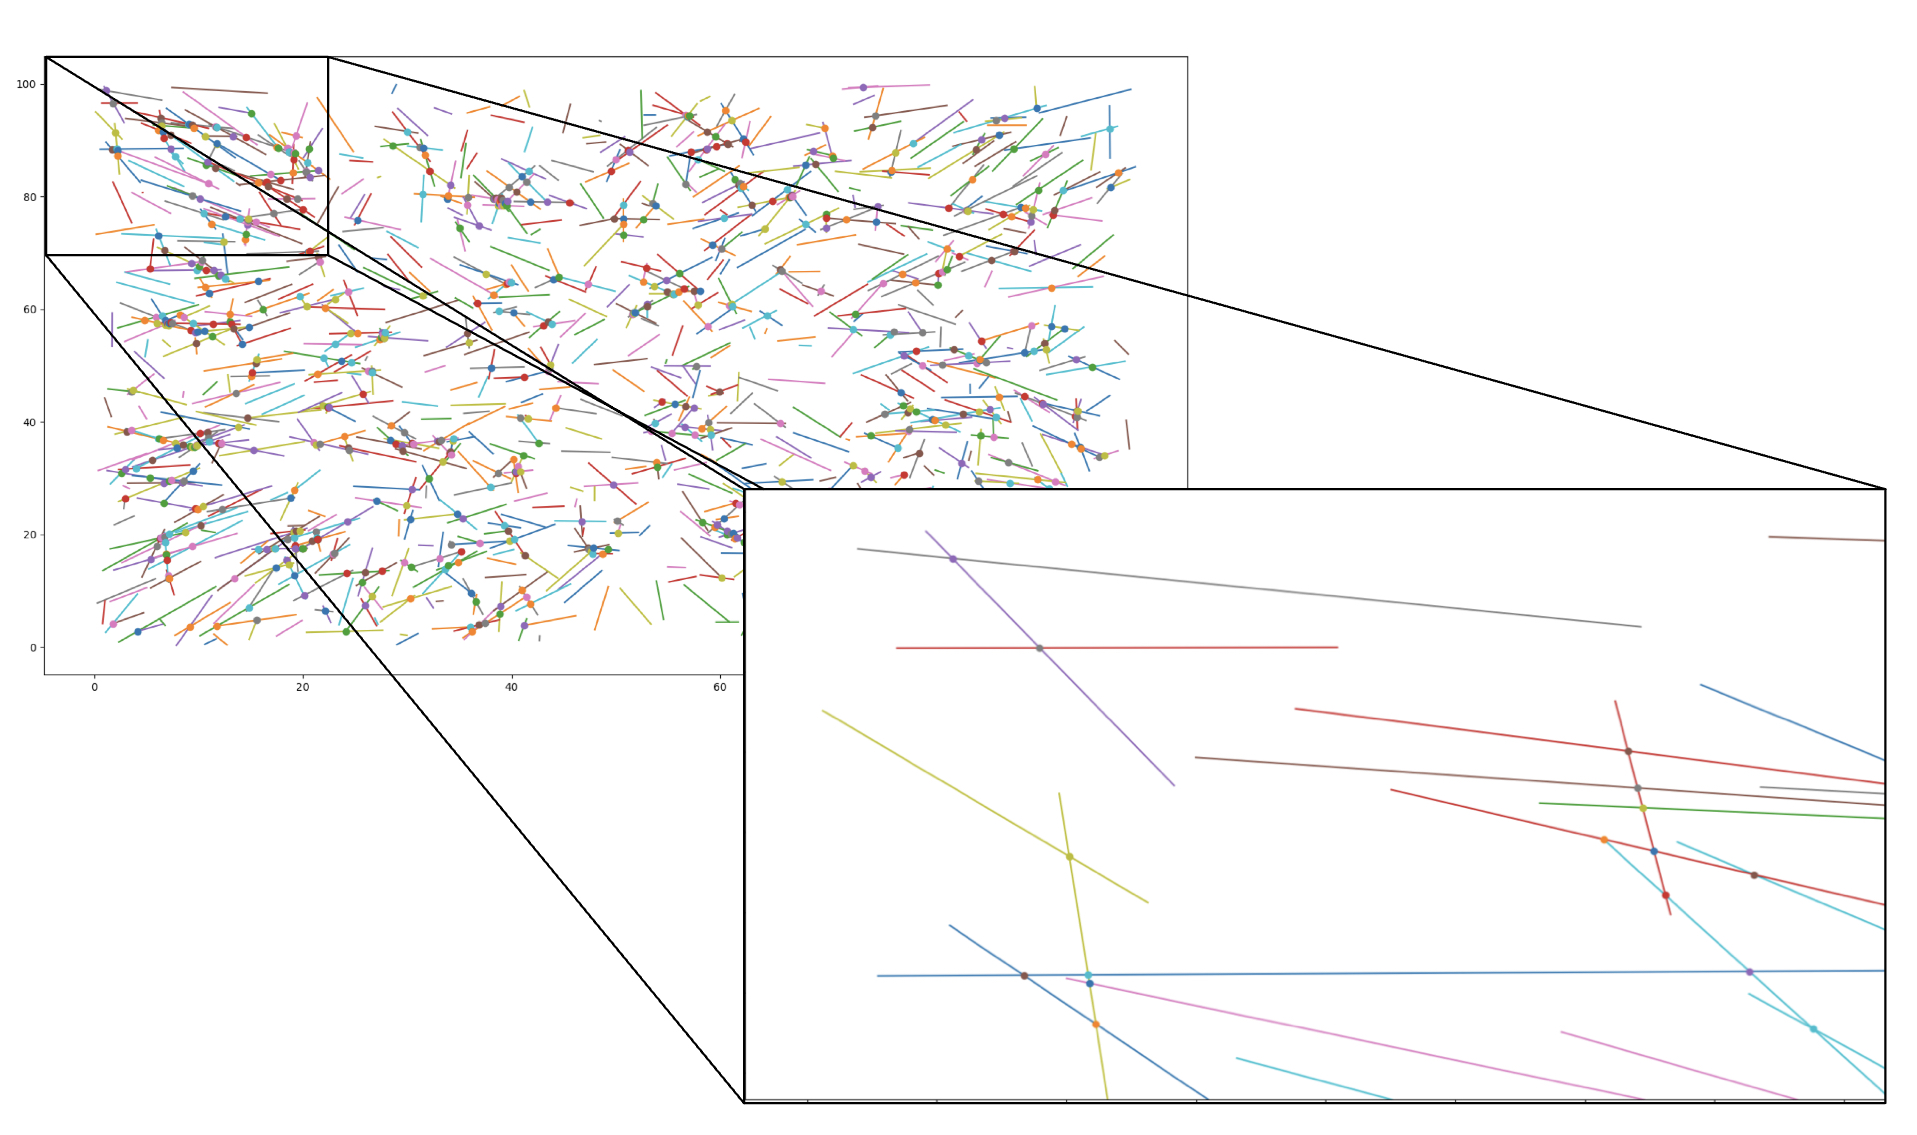
\includegraphics[scale=0.25]{Plot_zoom_and_all.jpeg}
%\end{figure}

%\begin{lstlisting}[style=Terminal, caption={testing.cpp: Ausgabe Konsole},captionpos=b, label={lst:ausgabe_test}]
%\end{lstlisting}



\end{document}
